\documentclass[10pt,a4paper]{article}
\usepackage[utf8]{inputenc}
\usepackage[T1]{fontenc}
\usepackage[margin=1.9cm]{geometry}
\usepackage{lmodern}
\usepackage{amsmath,amssymb}
\usepackage{booktabs,longtable,array,tabularx}
\usepackage{graphicx}
\usepackage{float}
\usepackage{xcolor}
\usepackage{listings}
\usepackage[hidelinks]{hyperref}
\usepackage{enumitem}
\usepackage{multicol}
\setlength{\parskip}{2pt}
\setlength{\abovecaptionskip}{3pt}
\setlength{\belowcaptionskip}{0pt}
\raggedbottom
\setlist{itemsep=0pt,topsep=2pt,parsep=0pt}

\newcommand{\code}[1]{\texttt{\detokenize{#1}}}
\newcommand{\todo}[1]{\textcolor{red}{\textbf{[#1]}}}

\lstset{
  basicstyle=\ttfamily\footnotesize,
  breaklines=true,
  breakatwhitespace=false,
  columns=fullflexible,
  keepspaces=true,
  frame=single,
  rulecolor=\color{black!30},
  xleftmargin=2pt,xrightmargin=2pt,
  showstringspaces=false
}

\title{\textbf{DAS 839 -- NoSQL Systems, Assignment II}\\[2pt]
\large MapReduce: Word Association, Document Indexing, Query Retrieval and Scalability}
\author{%
\begin{tabular}{@{}ccc@{}}
KM Yashaswini (BT2024224) & Vishal Reddy Kondakindi (BT2024102) & Shrey Modi (BT2024125)\
{\small Person 1} & {\small Person 2} & {\small Person 3}\[3pt]
\multicolumn{3}{c}{Abhinav Ravi (BT2024239) \small --- Person 4}\
\end{tabular}\[3pt]
{\small Repository: \url{https://github.com/yashaswini450/NoSQL-2}}}
\date{}

\begin{document}
\setlength{\abovedisplayskip}{3pt}\setlength{\belowdisplayskip}{3pt}
\vspace{-4pt}\maketitle\vspace{-10pt}

\begin{abstract}\small\noindent
All parts were implemented on Apache Hadoop 3.4.3 and run on the full corpus \code{Wikipedia-EN-20120601_ARTICLES} (10{,}000 articles).
Problem~1: top-50 frequent words, Pairs and Stripes word association ($d=2$), and a scalability study of four configurations on nested subsets (10--100\%).
Problem~2: stemmed document frequency, top-100 inverted index, and TF--IDF query retrieval. All numbers come from our own runs; logs and outputs are in the repository.
\end{abstract}


%=====================================================================
\section{Environment and setup}
%=====================================================================
\subsection{Software and hardware}
Everything ran in standalone (local) Hadoop mode: LocalJobRunner on the local filesystem, no HDFS and
no YARN. The jobs were run on three different laptops (each teammate ran their own part), so the
hardware is listed per part. Timings are therefore only comparable \emph{within} one experiment.

\begin{table}[H]\centering\small
\begin{tabularx}{\textwidth}{@{}l X X X@{}}
\toprule
 & Problem 1(d) benchmark (Person~2) & Problem 2(a) (Person~3) & Problem 2(b) (Person~4)\\
\midrule
OS & Windows~11, WSL2 Ubuntu, Linux 6.6.87.2 & Windows~11, WSL2 Ubuntu, Linux 6.18.54.1 & Windows~11, WSL2 Ubuntu, Linux 6.18.33.2\\
CPU & AMD Ryzen 7 7735HS, 16 logical CPUs & AMD Ryzen 9 6900HS, 16 logical CPUs & Intel Core i5-12450H, 12 logical CPUs\\
RAM seen by WSL & 7.4~GiB & 7.4~GiB & about 7~GiB\\
Java & Corretto OpenJDK 11.0.33 & Temurin OpenJDK 11.0.33 & OpenJDK 11.0.32\\
Hadoop & 3.4.3 standalone & 3.4.3 standalone & 3.4.3 standalone\\
JVM heap & \code{-Xmx1g} & default & default\\
\bottomrule
\end{tabularx}
\caption{Execution environments. \todo{Person~1: add the machine used for the original 1(a)/1(b) run; Person~2 reproduced 1(a)/1(b) on the machine in column 1 and all benchmark numbers come from it.}}
\end{table}

Other libraries: \code{opennlp-tools-1.9.3.jar} (\code{PorterStemmer}, Problem~2), Python~3 with
Matplotlib (plotting) and standard-library scripts for the independent checks.

\subsection{Dataset preparation}
\begin{itemize}
 \item \code{Wikipedia-EN-20120601_ARTICLES.tar.gz} is, despite its name, a plain tar archive (\code{tar -xf}).
 It contains \textbf{10{,}000} articles, one file \code{<id>.txt} each, 166{,}222{,}646 bytes. Each article is one line.
 The test set \code{Wikipedia-50-ARTICLES.tar} (50 articles, 717{,}789 bytes) was used for development only.
 \item \code{stopwords.txt} has 355 non-empty entries (47 contain an apostrophe and can never match a token after
 splitting on non-alphanumerics; we kept the official list unchanged).
 \item \textbf{Document ID} = article file name without \code{.txt}, a stable integer.
\end{itemize}

\subsection{Nested deterministic subsets (Problem 1(d))}
\code{prepare_subsets.sh} sorts the \code{.txt} file names by byte order and takes the first
$\lfloor N\cdot p/100\rfloor$ files for $p\in\{10,20,40,80,100\}$, so
$S_{10}\subset S_{20}\subset S_{40}\subset S_{80}\subset S_{100}$. The selected articles are written, in order, into
about 16~MiB text shards (to avoid one map task per small file); a newline is added where needed so that no
co-occurrence window crosses an article boundary.

\begin{table}[H]\centering\small
\begin{tabular}{@{}rrrr@{}}
\toprule
Subset & Documents & Source bytes & Hadoop input bytes\\
\midrule
10\%  & 1{,}000  & 11{,}021{,}771  & 11{,}022{,}771\\
20\%  & 2{,}000  & 27{,}653{,}453  & 27{,}655{,}453\\
40\%  & 4{,}000  & 64{,}709{,}490  & 64{,}713{,}490\\
80\%  & 8{,}000  & 130{,}964{,}811 & 130{,}972{,}811\\
100\% & 10{,}000 & 166{,}222{,}646 & 166{,}232{,}646\\
\bottomrule
\end{tabular}
\caption{Subsets (\code{subsets.tsv}); the difference is the added newlines.}
\end{table}

%=====================================================================
\section{Design and implementation}
%=====================================================================
\subsection{Common conventions}
All problems use the same text pipeline. Case normalisation: lowercase. Tokenisation: split on
\code{[^a-z0-9]+} (punctuation, apostrophes and non-ASCII letters are separators); empty tokens are dropped.
Stop words are read from \code{stopwords.txt} shipped through Hadoop's DistributedCache and loaded into a
\code{HashSet} in \code{Mapper.setup()}; a token is skipped if it is in the set (this replaces the
substring \code{replaceAll} of the starter \code{WordCount2.java}, which corrupts words). Problem~2 additionally applies the
OpenNLP \code{PorterStemmer} \emph{after} stop-word removal (\code{TextPreprocessor.terms()}, shared by 2(a) and 2(b)).
Ties are always broken by ascending lexicographic order of the word/term (numeric order of DOC\_ID for documents).

\subsection{Problem 1(a): top-50 frequent words (\code{Top50Words.java})}
Map emits $(w,1)$ per non-stop token; a combiner sums per split; a single reducer accumulates corpus totals and, in
\code{cleanup()}, sorts by (frequency desc, word asc) and writes the first 50 as \code{WORD<TAB>FREQUENCY}.
\begin{lstlisting}
setup():   stopwords <- cached stopwords.txt
map(k, line):  for token in line.toLowerCase().split("[^a-z0-9]+"):
                   if token != "" and token not in stopwords: emit(token, 1)
combine/reduce(w, counts): total[w] <- sum(counts)
cleanup(): sort total by (count desc, w asc); emit first 50
\end{lstlisting}

\subsection{Problem 1(b): Pairs (\code{WordAssociationPairs.java})}
The vocabulary $V_{50}$ (\code{top50_words.tsv}) is loaded from the cache. For each line the filtered
(non-stop) token stream $t_0,\dots,t_{n-1}$ is scanned; for every position $i$ with $t_i\in V_{50}$, each neighbour $t_j$ with
$1\le|i-j|\le d=2$ and $t_j\in V_{50}$, $t_j\ne t_i$, emits the \emph{ordered} pair $(u,v)=(t_i,t_j)$ with count~1.
Non-vocabulary tokens keep their positions (the window counts filtered tokens, not only vocabulary words). Pairs are
\textbf{ordered}, $C(u,v)=C(v,u)$ holds by symmetry of the window, self-pairs are excluded from counts and denominators.
The reducer sums $C(u,v)$, computes $\sum_{w}C(u,w)$ and
$P(v\mid u)=C(u,v)/\sum_w C(u,w)$, and keeps the 5 largest $C(u,v)$ per $u$ (ties by $v$ ascending).
Local-aggregation modes: \code{false}/none (emit every co-occurrence), \code{function} (aggregate in a per-record
\code{HashMap} flushed at the end of \code{map()}), and \code{true}/class (in-mapper \code{HashMap} across the whole split,
flushed once in \code{cleanup()} and cleared, plus a \code{PairsCombiner}).

\subsection{Problem 1(c): Stripes (\code{WordAssociationStripes.java})}
Same tokenisation, window, vocabulary and ordered-pair convention as Pairs. For each focal occurrence $u\in V_{50}$ the mapper
builds a stripe, a map $v\mapsto$ count of its neighbours in the window. Without aggregation each non-empty stripe is emitted
immediately as $(u,\text{stripe})$ (\code{MapWritable}); with aggregation one stripe per word is kept for the whole split
and emitted in \code{cleanup()} (state is bounded by $|V_{50}|=50$). The reducer merges stripes, computes the
denominator and $P(v\mid u)$ exactly as in Pairs and writes the same schema
(\code{u<TAB>v<TAB>C(u,v)<TAB>P(v|u)}, six decimals).

\subsection{Problem 1(d): local aggregation and scalability}
\code{run_scalability.sh} runs Pairs and Stripes, each with aggregation off and on (four configurations), one job at a
time, on the five nested subsets with $d=2$ and the same top-50 vocabulary. 10\%, 40\% and 100\% are run three times,
20\% and 80\% once. Wall-clock time is measured from just before the job launch until the process exits (JVM startup,
job, and output writing; not extraction, subset preparation or compilation). Mapper-output records and bytes are read from the
Hadoop counters. \code{plot_scalability.py} draws input size vs.\ runtime.

\subsection{Problem 2(a): DF and inverted index (\code{DocumentFrequency.java}, \code{InvertedIndex.java})}
A custom \code{WholeDocumentInputFormat} (a \code{CombineFileInputFormat}) returns one record per article, so each
\code{map()} call sees exactly one document, and files are combined into splits of at most 64~MB (3 map tasks instead of 10{,}000).
\begin{lstlisting}
Job 1 (DF):   map(docId, text): for t in set(terms(text)): emit(t, 1)     # once per doc
              combine = reduce: emit(t, sum)                               # = DF(t)
Job 2 (top100): each mapper keeps a TreeSet ordered by (df desc, term asc), size 100,
              emits it in cleanup(); one reducer merges to the global top 100.
InvertedIndex: map(docId, text): tf <- count of each top-100 term in text;
                                 for (t,c) in tf: emit(t, docId ":" c)
               reduce(t, postings): sort by numeric docId; emit(t, "d1:tf1,d2:tf2,...")
\end{lstlisting}
DF counts \emph{distinct documents} (a term used 50 times in one article counts once). Because every combiner value is one
distinct (term, document) pair, summing early cannot double-count. Top-100 ties: DF descending, then TERM ascending.
Output schemas: \code{TERM<TAB>DF}; \code{TERM<TAB>DOC_ID:TF,DOC_ID:TF,...}.

\subsection{Problem 2(b): query retrieval (\code{QueryRetrieval.java})}
\paragraph{Inputs.} \code{inverted_index.tsv} (MapReduce input), \code{top100_df.tsv} (DistributedCache; source of DF),
$N$ (from \code{doc_count.txt}), \code{stopwords.txt}, and the query string.
\paragraph{Query handling (driver).}
\begin{enumerate}
 \item The query goes through the \emph{same} pipeline as the documents (\code{TextPreprocessor.terms()}).
 \item \textbf{Repeated query terms} collapse into the \emph{set} $Q$ (matching $t\in Q\cap D$); the score is not multiplied by query multiplicity.
 \item Stop words disappear in step~1. Terms \textbf{absent from the index} (not among the 100 indexed terms) are logged as ignored and skipped.
 \item If no usable term remains (e.g.\ only stop words), the driver prints ``no documents can match'', runs no job and writes no output.
 If usable terms exist but no document contains them, the output is empty.
\end{enumerate}
\paragraph{Scoring.} $\mathrm{IDF}(t)=\ln\!\bigl(N/\mathrm{DF}(t)+1\bigr)$ (natural log), $S(D,Q)=\sum_{t\in Q\cap D}\mathrm{TF}(t,D)\cdot\mathrm{IDF}(t)$.
The formula is used unchanged (no length normalisation).
\begin{lstlisting}
driver:  Q <- set(terms(query)) intersect indexedTerms(top100_df.tsv); if Q empty: report, exit
         conf: Q, N; cacheFile: top100_df.tsv; 1 reducer
setup(): dfByTerm <- cached top100_df.tsv
map(line "TERM \t d1:tf1,d2:tf2,..."):
    if TERM not in Q: return
    idf <- ln(N / dfByTerm[TERM] + 1)
    for each posting d:tf: emit(d, TERM ":" tf*idf)
    if #postings != dfByTerm[TERM]: counter DF_MISMATCH++       # consistency with 2(a)
reduce(doc, values):  perTerm <- TreeMap(term -> contribution)  # summed in term order
    hit <- (sum of contributions, sorted matched terms)
cleanup():  sort hits by score desc, then DOC_ID asc (numeric); write top 10:
            RANK \t DOC_ID \t MATCHED_TERMS \t SCORE (6 decimals)
\end{lstlisting}
\paragraph{Design decisions.} (i) DF is read from Part~2(a)'s \code{top100_df.tsv}, as the assignment requires, and cross-checked against the
posting count. (ii) Tie-breaking: equal scores are ordered by DOC\_ID ascending, \emph{compared numerically} (so 999 precedes 1000);
contributions are summed in sorted-term order, so floating-point sums do not depend on shuffle order. (iii) One reducer gives a global top-10;
at most $N$ candidate documents fit in memory.

%=====================================================================
\section{Correctness checks}
%=====================================================================
\subsection{Problem 1(a): top-50 words}
All 50 words in \code{top50_words.tsv} were checked against \code{stopwords.txt}: \textbf{0} stop words appear. The ranking uses
(frequency desc, word asc), so ties are deterministic. Person~2 reproduced the same 50 words and frequencies by re-running
\code{Top50Words} on the prepared corpus, and an independent Python recount from the raw article files agreed.

\begin{table}[H]\centering\small
\begin{tabular}{@{}rlr@{\hspace{2em}}rlr@{}}
\toprule
\# & word & frequency & \# & word & frequency\\
\midrule
1 & apos & 273{,}057 & 6 & 2 & 66{,}358\\
2 & quot & 267{,}968 & 7 & category & 60{,}534\\
3 & s & 207{,}334 & 8 & this & 58{,}764\\
4 & http & 79{,}108 & 9 & 0 & 54{,}719\\
5 & 1 & 77{,}032 & 10 & www & 54{,}136\\
\bottomrule
\end{tabular}
\caption{First ten rows of \code{top50_words.tsv}. Words such as \code{apos}, \code{quot} (HTML entities), \code{http}, \code{www} and bare numbers appear because the agreed tokenizer does not filter them (see Section~6).}
\end{table}

\subsection{Problems 1(b) and 1(c): Pairs vs.\ Stripes and aggregation modes}
\begin{itemize}
 \item The three Pairs modes (none / function / class) produce identical \code{pairs_top5.tsv} (\code{diff -u} clean, 250 rows = 5 associations $\times$ 50 words).
 \item \code{diff pairs_top5.tsv stripes_top5.tsv} is empty: \textbf{Stripes reproduces Pairs exactly} (counts and probabilities). This was re-checked on the merged \code{main}.
 \item Within the benchmark, all four configurations produced identical output at every subset size and trial, and an independent recount from the original articles matched at all five sizes.
 \item Symmetry sanity check: $C(\text{united},\text{states})=C(\text{states},\text{united})=21{,}734$, yet
 $P(\text{states}\mid\text{united})=0.664059\neq P(\text{united}\mid\text{states})=0.685507$ because the denominators differ.
\end{itemize}

\begin{table}[H]\centering\small
\begin{tabular}{@{}lrrr@{}}
\toprule
$u$ & $v$ & $C(u,v)$ & $P(v\mid u)$\\
\midrule
united & states   & 21734 & 0.664059\\
united & category & 2475  & 0.075621\\
united & county   & 946   & 0.028904\\
united & quot     & 804   & 0.024565\\
united & 1        & 688   & 0.021021\\
\bottomrule
\end{tabular}
\caption{Top-5 associations of ``united'' (rows of \code{pairs_top5.tsv}).}
\end{table}

\subsection{Problem 2(a): DF and inverted index}
\code{check_problem2a.py} (plain Python, independent of the Java code and of the stemmer) reports \textbf{ALL CHECKS PASSED} on the full corpus:
$N=10{,}000$ equals the number of files; \code{df_all.tsv} (524{,}390 terms) has no duplicate term and $1\le\mathrm{DF}\le N$;
\code{top100_df.tsv} equals the true top~100 of \code{df_all.tsv} under (DF desc, TERM asc); the boundary DF 4832 at rank 100 is held by a single term (no tie excluded);
the index holds exactly the 100 terms; \textbf{number of postings equals DF for every term}, so no document is counted twice;
no duplicate DOC\_ID inside a posting list; every TF$\ge1$; postings sorted. A raw-text cross-check for 12 terms unchanged by stemming
(e.g.\ \code{american}, \code{first}, \code{form}) found every article containing the raw token in the postings with TF at least the raw count.
Hand checks with \code{grep} on the 50-article set: \code{includ} DF 42 (grep 42), \code{peopl} DF 36 (grep 36), TF of \code{includ} in doc 1338 = 12 (grep 12).
Stop words cannot appear: they are removed before stemming and no top-100 term is spelled like a stop word.

\begin{table}[H]\centering\small
\begin{tabular}{@{}rlr@{\hspace{2em}}rlr@{}}
\toprule
rank & term & DF & rank & term & DF\\
\midrule
1 & s & 9836 & 6 & other & 8415\\
2 & apo & 9518 & 7 & 1 & 8350\\
3 & categori & 9381 & 8 & link & 8295\\
4 & refer & 9340 & 9 & thi & 8190\\
5 & quot & 8674 & 10 & 2 & 8105\\
\bottomrule
\end{tabular}
\caption{Top-10 terms by DF (full list in \code{top100_df.tsv}; rank 100 is \code{major}, DF 4832).}
\end{table}

Representative inverted-index records (first 10 postings; \code{s 698:39} means ``term \code{s} occurs 39 times in article 698''):
\begin{lstlisting}
s      698:39,700:95,708:2,709:8,740:10,842:7,857:8,864:148,900:44,902:91
major  698:8,700:3,709:2,740:2,842:1,864:2,902:2,1178:1,1198:3,1214:4
\end{lstlisting}

\subsection{Problem 2(b): query ranking}
\paragraph{Query used.} No instructor-supplied query had been announced, so we used our own multi-term query
\textbf{``history united states''}. It becomes $Q=\{\text{histori},\text{state},\text{unit}\}$ (none of the three words is a stop word). $N=10{,}000$.
The program accepts any query; another query needs only a re-run of \code{run_query.sh}.

\begin{table}[H]\centering\small
\begin{tabular}{@{}lrr@{}}
\toprule
Term $t$ & DF$(t)$ (\code{top100_df.tsv}) & IDF$(t)=\ln(10000/\mathrm{DF}+1)$\\
\midrule
histori & 6657 & 0.917162\\
state   & 7299 & 0.862911\\
unit    & 6498 & 0.931745\\
\bottomrule
\end{tabular}
\end{table}

9{,}018 documents contain at least one query term. Output of the Hadoop job (\code{query_top10.tsv}):

\begin{table}[H]\centering\small
\begin{tabular}{@{}rrlr@{}}
\toprule
RANK & DOC\_ID & MATCHED\_TERMS & SCORE\\
\midrule
1 & 334701 & state,unit & 580.808168\\
2 & 462443 & histori,state,unit & 384.904727\\
3 & 317144 & state,unit & 298.119407\\
4 & 31655  & histori,state,unit & 241.365556\\
5 & 18858  & histori,state,unit & 236.636569\\
6 & 201936 & histori,state,unit & 236.551865\\
7 & 62513  & histori,state,unit & 234.387576\\
8 & 21650  & histori,state,unit & 230.939936\\
9 & 560898 & state,unit & 212.701161\\
10 & 225102 & histori,state,unit & 208.959599\\
\bottomrule
\end{tabular}
\end{table}

\paragraph{Worked score calculations} (TF from \code{inverted_index.tsv}, IDF from the table above; products rounded, totals in double precision):
\begin{align*}
S(334701,Q) &= 672\times0.862911 + 1\times0.931745 = 579.876423+0.931745 = \mathbf{580.808168}\\
S(462443,Q) &= 1\times0.917162+215\times0.862911+213\times0.931745 = 0.917162+185.525939+198.461626 = \mathbf{384.904727}\\
S(317144,Q) &= 163\times0.862911+169\times0.931745 = 140.654549+157.464858 = \mathbf{298.119407}
\end{align*}

\paragraph{Validation.}
(i) \code{verify_retrieval.py}, a Hadoop-free re-implementation that reads DF from \code{top100_df.tsv}, gives output \emph{identical} to the Hadoop job
on the full corpus (and on the 50-article set, $N=50$, top document 1338 with score 46.733929).
(ii) The counter \code{DF_MISMATCH} never fired: the posting count equals DF for every queried term.
(iii) Edge cases that were run: a stop-word-only query (\code{the of and}) $\to$ no terms, message, no job;
\code{zzzqqq history history History} $\to$ \code{zzzqqq} ignored as absent, repeated \code{history} collapsed, ranking by \code{histori} only;
documents 7174 and 45633 have exactly equal scores (72.455768) and are ordered numerically.

\paragraph{Why this ranking is reasonable (and its limits).}
The formula is applied exactly as specified: raw TF$\times$IDF, no length normalisation. All three query terms are very common
(DF 65--73\% of the corpus), so their IDFs are low and almost equal (0.86--0.93) and \textbf{TF dominates} the score.
Hence the top document (334701, a long list of numbered New York \emph{state} highways) does not contain ``histori'' at all: it uses ``state'' 672 times.
Documents 462443 (a US-Congress table with 215 ``state'', 213 ``unit'') and 317144 (an airport list with many ``United States'' entries)
are likewise repetition-driven, while documents matching all three terms fill ranks 4--8 and 10. This is a property of the specified scoring
function (long, repetitive documents win; very common terms discriminate poorly), not of the implementation, and we did not change the formula.

%=====================================================================
\section{Performance evaluation}
%=====================================================================
\subsection{Problem 1(d): scalability study}
Machine: Person~2's laptop (Table~1, column~1), standalone Hadoop, one job at a time, one reducer.
Cells for 10\%, 40\% and 100\% are the \textbf{median of three runs}; 20\% and 80\% are single runs (as required).
Sizes are the actual Hadoop input bytes.

\begin{table}[H]\centering\small
\begin{tabular}{@{}rrrrrrr@{}}
\toprule
Subset & Docs & MiB & Pairs-NoAgg (s) & Pairs-Agg (s) & Stripes-NoAgg (s) & Stripes-Agg (s)\\
\midrule
10\%  & 1{,}000  & 10.51  & 7.64  & 7.70  & 8.70  & 7.77\\
20\%  & 2{,}000  & 26.37  & 11.70 & 10.84 & 12.95 & 10.94\\
40\%  & 4{,}000  & 61.72  & 17.88 & 16.33 & 19.77 & 16.17\\
80\%  & 8{,}000  & 124.91 & 35.58 & 28.51 & 33.71 & 27.30\\
100\% & 10{,}000 & 158.53 & 34.27 & 30.49 & 38.44 & 30.24\\
\bottomrule
\end{tabular}
\caption{Wall-clock runtime (seconds). All 44 individual measurements are in \code{scalability_runs.csv}.}
\end{table}

\begin{figure}[H]\centering
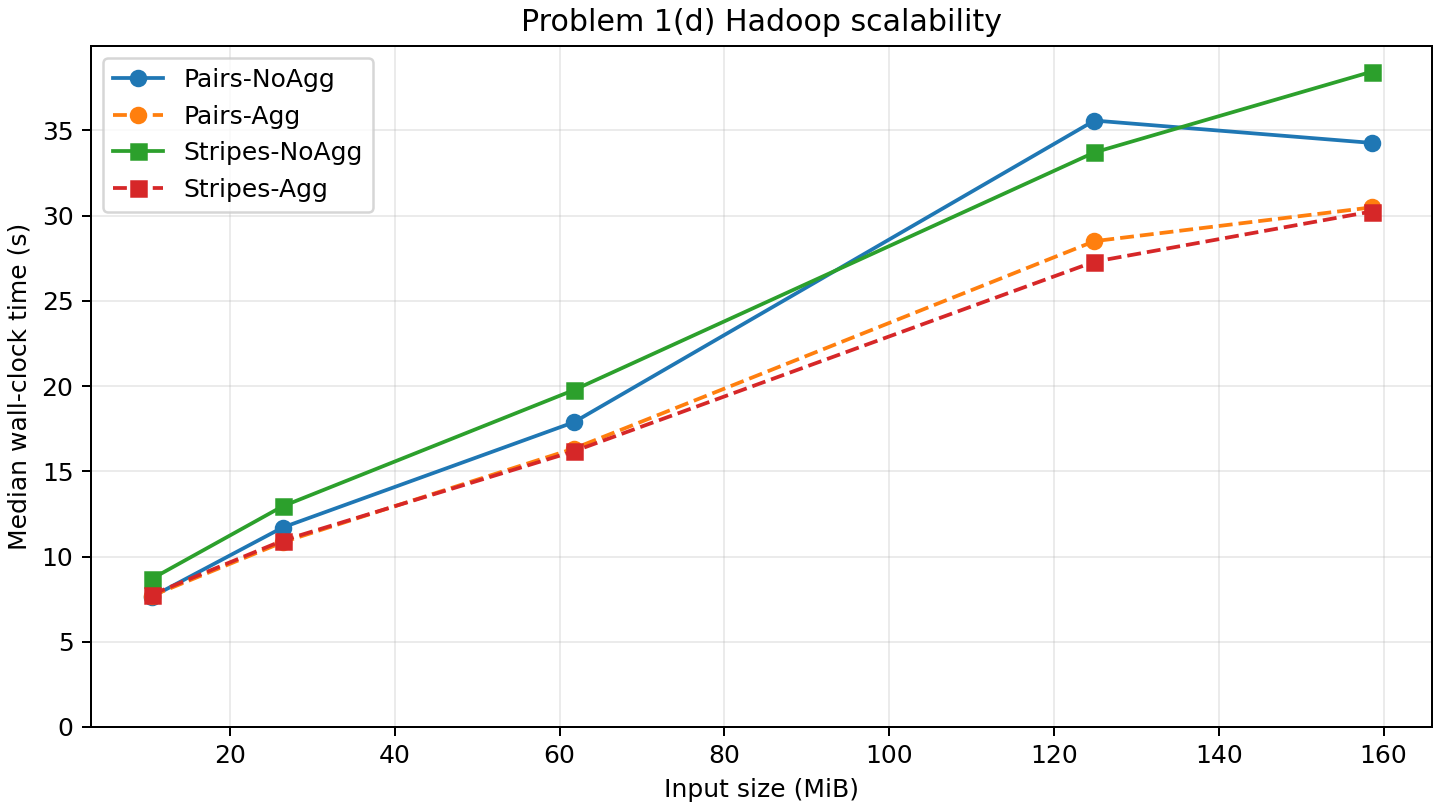
\includegraphics[width=0.62\textwidth]{scalability.png}
\caption{Input size vs.\ runtime for the four configurations (\code{scalability.png}).}
\end{figure}

\begin{table}[H]\centering\small
\begin{tabular}{@{}lrrrr@{}}
\toprule
 & \multicolumn{2}{c}{Median map output records} & \multicolumn{2}{c}{Median map output bytes}\\
Configuration & 10\% & 100\% & 10\% & 100\%\\
\midrule
Pairs-NoAgg    & 139{,}578 & 1{,}540{,}824 & 2{,}214{,}954 & 24{,}567{,}766\\
Pairs-Agg      & 2{,}280   & 23{,}526      & 38{,}020      & 392{,}606\\
Stripes-NoAgg  & 103{,}663 & 1{,}169{,}590 & 2{,}810{,}697 & 31{,}272{,}291\\
Stripes-Agg    & 50        & 500           & 33{,}159      & 342{,}149\\
\bottomrule
\end{tabular}
\caption{Intermediate data (Hadoop counters \code{Map output records/bytes}; values for all five sizes are in \code{scalability_results.csv}).}
\end{table}

\paragraph{Analysis.}
\begin{itemize}
 \item \textbf{Trend.} Input grows $15.1\times$ from 10\% to 100\%, while runtime grows only $3.9\times$--$4.5\times$ across the configurations: runtime is
 clearly sub-proportional because JVM/Hadoop startup and output writing are a fixed cost that dominates the small runs (about 7.6~s at 10\%).
 The 80\% Pairs-NoAgg value (35.58~s) is above its 100\% median (34.27~s); the 80\% cells are single runs, so this is run-to-run noise on a laptop and not a real trend.
 \item \textbf{Local aggregation helps.} It reduces mapper output by orders of magnitude: Pairs from 1{,}540{,}824 to 23{,}526 records ($-98.5\%$; at most
 $50\cdot49=2450$ distinct ordered pairs per mapper and 10 map tasks) and Stripes from 1{,}169{,}590 to 500 records, i.e.\ 50 stripes per mapper ($-99.96\%$, bytes $-98.9\%$).
 Runtime improves by $11\%$ (Pairs) and $21\%$ (Stripes) at 100\%, and Stripes-Agg is the fastest at 30.24~s, just ahead of Pairs-Agg (30.49~s).
 \item \textbf{Pairs vs.\ Stripes without aggregation.} Stripes emits fewer records (1.17~M vs.\ 1.54~M) but more bytes (31.3~MB vs.\ 24.6~MB), since each record carries a map of neighbour counts; it was also slower (38.44~s vs.\ 34.27~s).
 \item The Pairs ``function'' mode (aggregation per record only) was measured by Person~1 on the full corpus: 674{,}998 map output records versus 1{,}540{,}824 without aggregation ($-56.2\%$), i.e.\ between no aggregation and full in-mapper aggregation.
 \item The mapper-byte counters count serialised emissions; shuffle bytes differ slightly (see \code{problem1_hadoop_counters.txt}).
\end{itemize}

\subsection{Problem 2: indexing and retrieval timings}
These are single runs in standalone mode (no timing study was required for Problem~2); each includes JVM and job start-up and output writing.

\begin{table}[H]\centering\small
\begin{tabular}{@{}lrr@{}}
\toprule
Job & 50 articles & 10{,}000 articles\\
\midrule
2(a) DF + top-100 (two chained jobs) & 3.73~s & 20.08~s\\
2(a) inverted index                   & 2.41~s & 11.97~s\\
2(b) query retrieval (end-to-end, incl.\ \code{javac}+\code{jar}) & -- & 12.4~s\\
\bottomrule
\end{tabular}
\end{table}
Counters (full corpus): DF job: 3 map tasks, 10{,}000 input records, 7{,}153{,}978 map output records, reduced to 524{,}390 terms; the combiner cut shuffle
records from 7.15~M to 0.72~M ($-89.9\%$). Index job: 615{,}076 postings. Query job: 100 index lines read, 20{,}454 map output records, 9{,}018 matching documents, 10 output rows.
The 2(b) input is only the 5.4~MB index (100 lines), which is why retrieval is cheap compared with building the index.

%=====================================================================
\section{Reproducibility}
%=====================================================================
\subsection{Repository layout}
\begin{table}[H]\centering\footnotesize
\begin{tabular}{@{}p{0.43\textwidth}p{0.5\textwidth}@{}}
\toprule
Files & Content\
\midrule
\code{Top50Words.java}, \code{top50_words.tsv} & 1(a) code and output\
\code{WordAssociationPairs.java}, \code{pairs_top5.tsv} & 1(b) code and output\
\code{WordAssociationStripes.java}, \code{stripes_top5.tsv} & 1(c) code and output\
\code{prepare_subsets.sh}, \code{run_scalability.sh}, \code{plot_scalability.py} & 1(d) scripts\
\code{scalability_results.csv}, \code{scalability_runs.csv}, \code{subsets.tsv}, \code{scalability.png} & 1(d) results\
\code{DocumentFrequency.java}, \code{InvertedIndex.java}, \code{TextPreprocessor.java}, \code{WholeDocumentInputFormat.java} & 2(a) code\
\code{results_full/}, \code{results_50/} & 2(a) outputs, logs, checks (full / test set)\
\code{QueryRetrieval.java}, \code{run_query.sh}, \code{verify_retrieval.py} & 2(b) code, runner, check\
\code{query_top10.tsv}, \code{results_2b/} & 2(b) output, worked scores, run log\
\code{problem_1.txt}, \code{problem_2.txt} & run instructions (reproduced below)\
\bottomrule
\end{tabular}
\end{table}

\subsection{Main commands}
\begin{lstlisting}
# Problem 1 (full instructions in problem_1.txt below)
hadoop jar problem1.jar Top50Words stopwords.txt <input_dir> out_top50 50
hadoop jar problem1.jar WordAssociationPairs   stopwords.txt top50_words.tsv <input_dir> out_pairs   <false|function|true> 2
hadoop jar problem1.jar WordAssociationStripes stopwords.txt top50_words.tsv <input_dir> out_stripes <false|true>
bash prepare_subsets.sh <articles_dir> subsets ; bash run_scalability.sh subsets stopwords.txt top50_words.tsv problem1.jar out_bench

# Problem 2
./run_problem2a.sh Wikipedia-EN-20120601_ARTICLES results_full
./run_query.sh results_full "history united states" output_query
python3 verify_retrieval.py results_full "histori,state,unit" --explain 3
\end{lstlisting}
Fixed configuration: window $d=2$; one reducer per job; Top-K 50 and 100; split size limit 64~MB for 2(a); \code{-Xmx1g} for the benchmark.

\subsection{Contents of \texttt{problem\_1.txt} and \texttt{problem\_2.txt}}
\lstset{frame=none,basicstyle=\fontsize{5.6}{6.6}\ttfamily,xleftmargin=0pt,xrightmargin=0pt}
\begin{multicols}{2}
\noindent\textbf{\small problem\_1.txt}\par\smallskip
\lstinputlisting{problem_1.txt}
\columnbreak
\noindent\textbf{\small problem\_2.txt}\par\smallskip
\lstinputlisting{problem_2.txt}
\end{multicols}
\lstset{frame=single,basicstyle=\ttfamily\footnotesize}

%=====================================================================
\section{Limitations}
%=====================================================================
\begin{itemize}
 \item \textbf{Different machines.} The three experiment groups ran on three laptops (Table~1). Timings are comparable only within one experiment; the scalability benchmark (the only timing study) comes entirely from one machine, in standalone mode, so HDFS/YARN effects, network shuffle and multi-node scaling were not measured.
 \item \textbf{Single runs where allowed.} 20\% and 80\% subsets and all Problem~2 timings are single runs. The 80\% Pairs-NoAgg point is slower than the 100\% median, which shows the noise level of such single measurements.
 \item \textbf{Non-content tokens.} The agreed tokenizer does not filter numbers, single letters, HTML-entity residue (\code{apos}, \code{quot}), URL parts (\code{http}, \code{www}) or interlanguage prefixes (\code{fr}, \code{pt}\dots). About 45 of the 100 top-DF terms and several top-50 words are such tokens. The official stop-word list also lacks words such as ``this'' and ``us''. We kept the official list and the agreed pipeline unchanged so that all parts stay consistent; filtering would have to be applied to indexing and queries together.
 \item \textbf{Retrieval scope.} 2(b) searches only the 100 highest-DF terms indexed in 2(a); other query terms are ignored, so a query made only of rarer terms returns nothing. This follows the assignment's definition of the index.
 \item \textbf{Ranking quality.} Scoring uses raw TF with no length normalisation, so long, repetitive documents and very common terms dominate (Section~3.4).
 \item \textbf{Query.} No instructor-supplied query was announced; the reported results use our own query. If one is announced, the result files must be regenerated with \code{run_query.sh}.
 \item \textbf{Stemming.} Porter stems are not always words (\code{categori}, \code{histori}); non-ASCII letters act as separators (``caf\'e'' becomes the token \code{caf}).
 \item \textbf{Launcher.} The benchmark jobs were launched through Hadoop's \code{RunJar} with explicit client jars (same for all configurations); the standard \code{hadoop jar} command runs the same jobs but may have different launcher overhead.
\end{itemize}

\end{document}
